\documentclass{beamer}
%\usetheme{Boadilla}

\title{Bayesian Optimization}
\author{Steven Jin}
\usepackage[utf8]{inputenc}
\usepackage{algpseudocode}
\usepackage{algorithm}
\usepackage[T1]{fontenc}
\usepackage{textcomp}
\usepackage[english]{babel}
\usepackage{verbatim}
\usepackage{cite}
%\setlist[enumerate]{ label=\arabic*.}


% Hide page number when page is empty
\usepackage{multicol}
\usepackage{xcolor}
% Other font I sometimes use.
% \usepackage{cmbright}

% Math stuff
\usepackage{amsmath, amsfonts, mathtools, amsthm, amssymb}
% Fancy script capitals
\usepackage{mathrsfs}
% Bold math
\usepackage{bm}


% Operators
\DeclareMathOperator{\Bd}{Bd}
\DeclareMathOperator{\Int}{Int}
\DeclareMathOperator{\cif}{if\;}

\DeclareMathOperator{\Var}{Var}
\DeclareMathOperator{\SD}{SD}
\DeclareMathOperator{\Cov}{Cov}
\DeclareMathOperator{\Cor}{Cor}
\DeclareMathOperator{\Pois}{Pois}
\DeclareMathOperator{\Dir}{Dir}
\DeclareMathOperator{\Unif}{Unif}
\DeclareMathOperator{\Gam}{Gamma}
\DeclareMathOperator{\Binom}{Binom}
\DeclareMathOperator{\Expo}{Expo}
\DeclareMathOperator{\dBeta}{dBeta}
\DeclareMathOperator{\tBeta}{tBeta}
\DeclareMathOperator{\Ber}{Ber}
\DeclareMathOperator{\IG}{IG}
\DeclareMathOperator{\Pb}{Pr}
\DeclareMathOperator*{\argmax}{arg\,max}
\DeclareMathOperator*{\argmin}{arg\,min}
\newcommand\deq{\stackrel{\mathclap{\tiny\mbox{d}}}{=}}
\def\bsy{\boldsymbol}



\begin{document}
\begin{frame}
    \titlepage
\end{frame}

\begin{frame}
    \frametitle{Motivation}
    \begin{columns}
        \begin{column}{0.5\textwidth}
            ``Why not the best?'' --Jimmy Carter
        \end{column}
        \begin{column}{0.5\textwidth}
            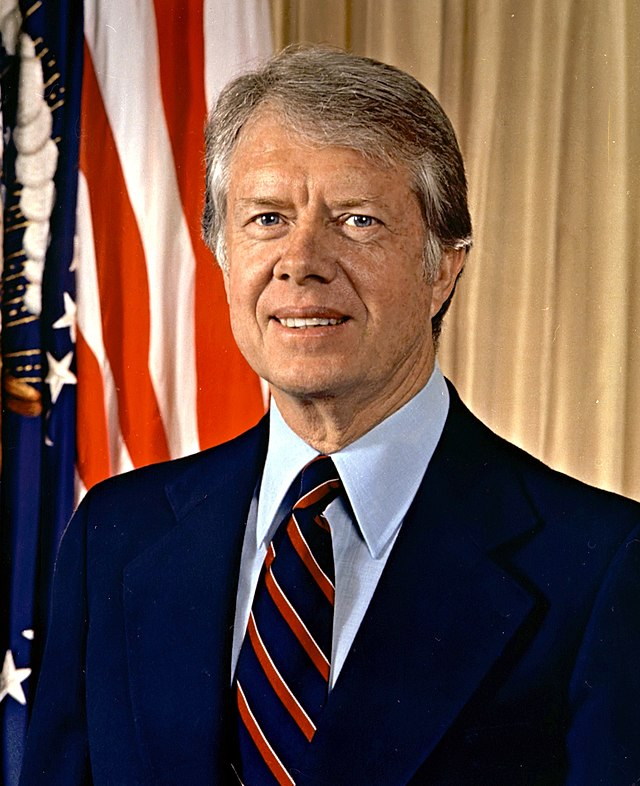
\includegraphics[width=\textwidth]{fig/JimmyCarterPortrait2.jpg}
        \end{column}
    \end{columns}
\end{frame}

\begin{frame}
    \frametitle{Motivation}
    How to maximize differentiable $f:[a, b] \to \mathbb{R}$?


    \begin{columns}
        \begin{column}{0.6\textwidth}
            \begin{enumerate}
                \pause
                \item solve $f'(c) = 0$.
                    \pause
                \item check $f''(c) \leq 0$.
                    \pause
                \item evaluate $f$ at $a$, $b$, and local maxes.
            \end{enumerate}
        \end{column}
        \pause
        \begin{column}{0.4\textwidth}
            \vspace{15pt}

            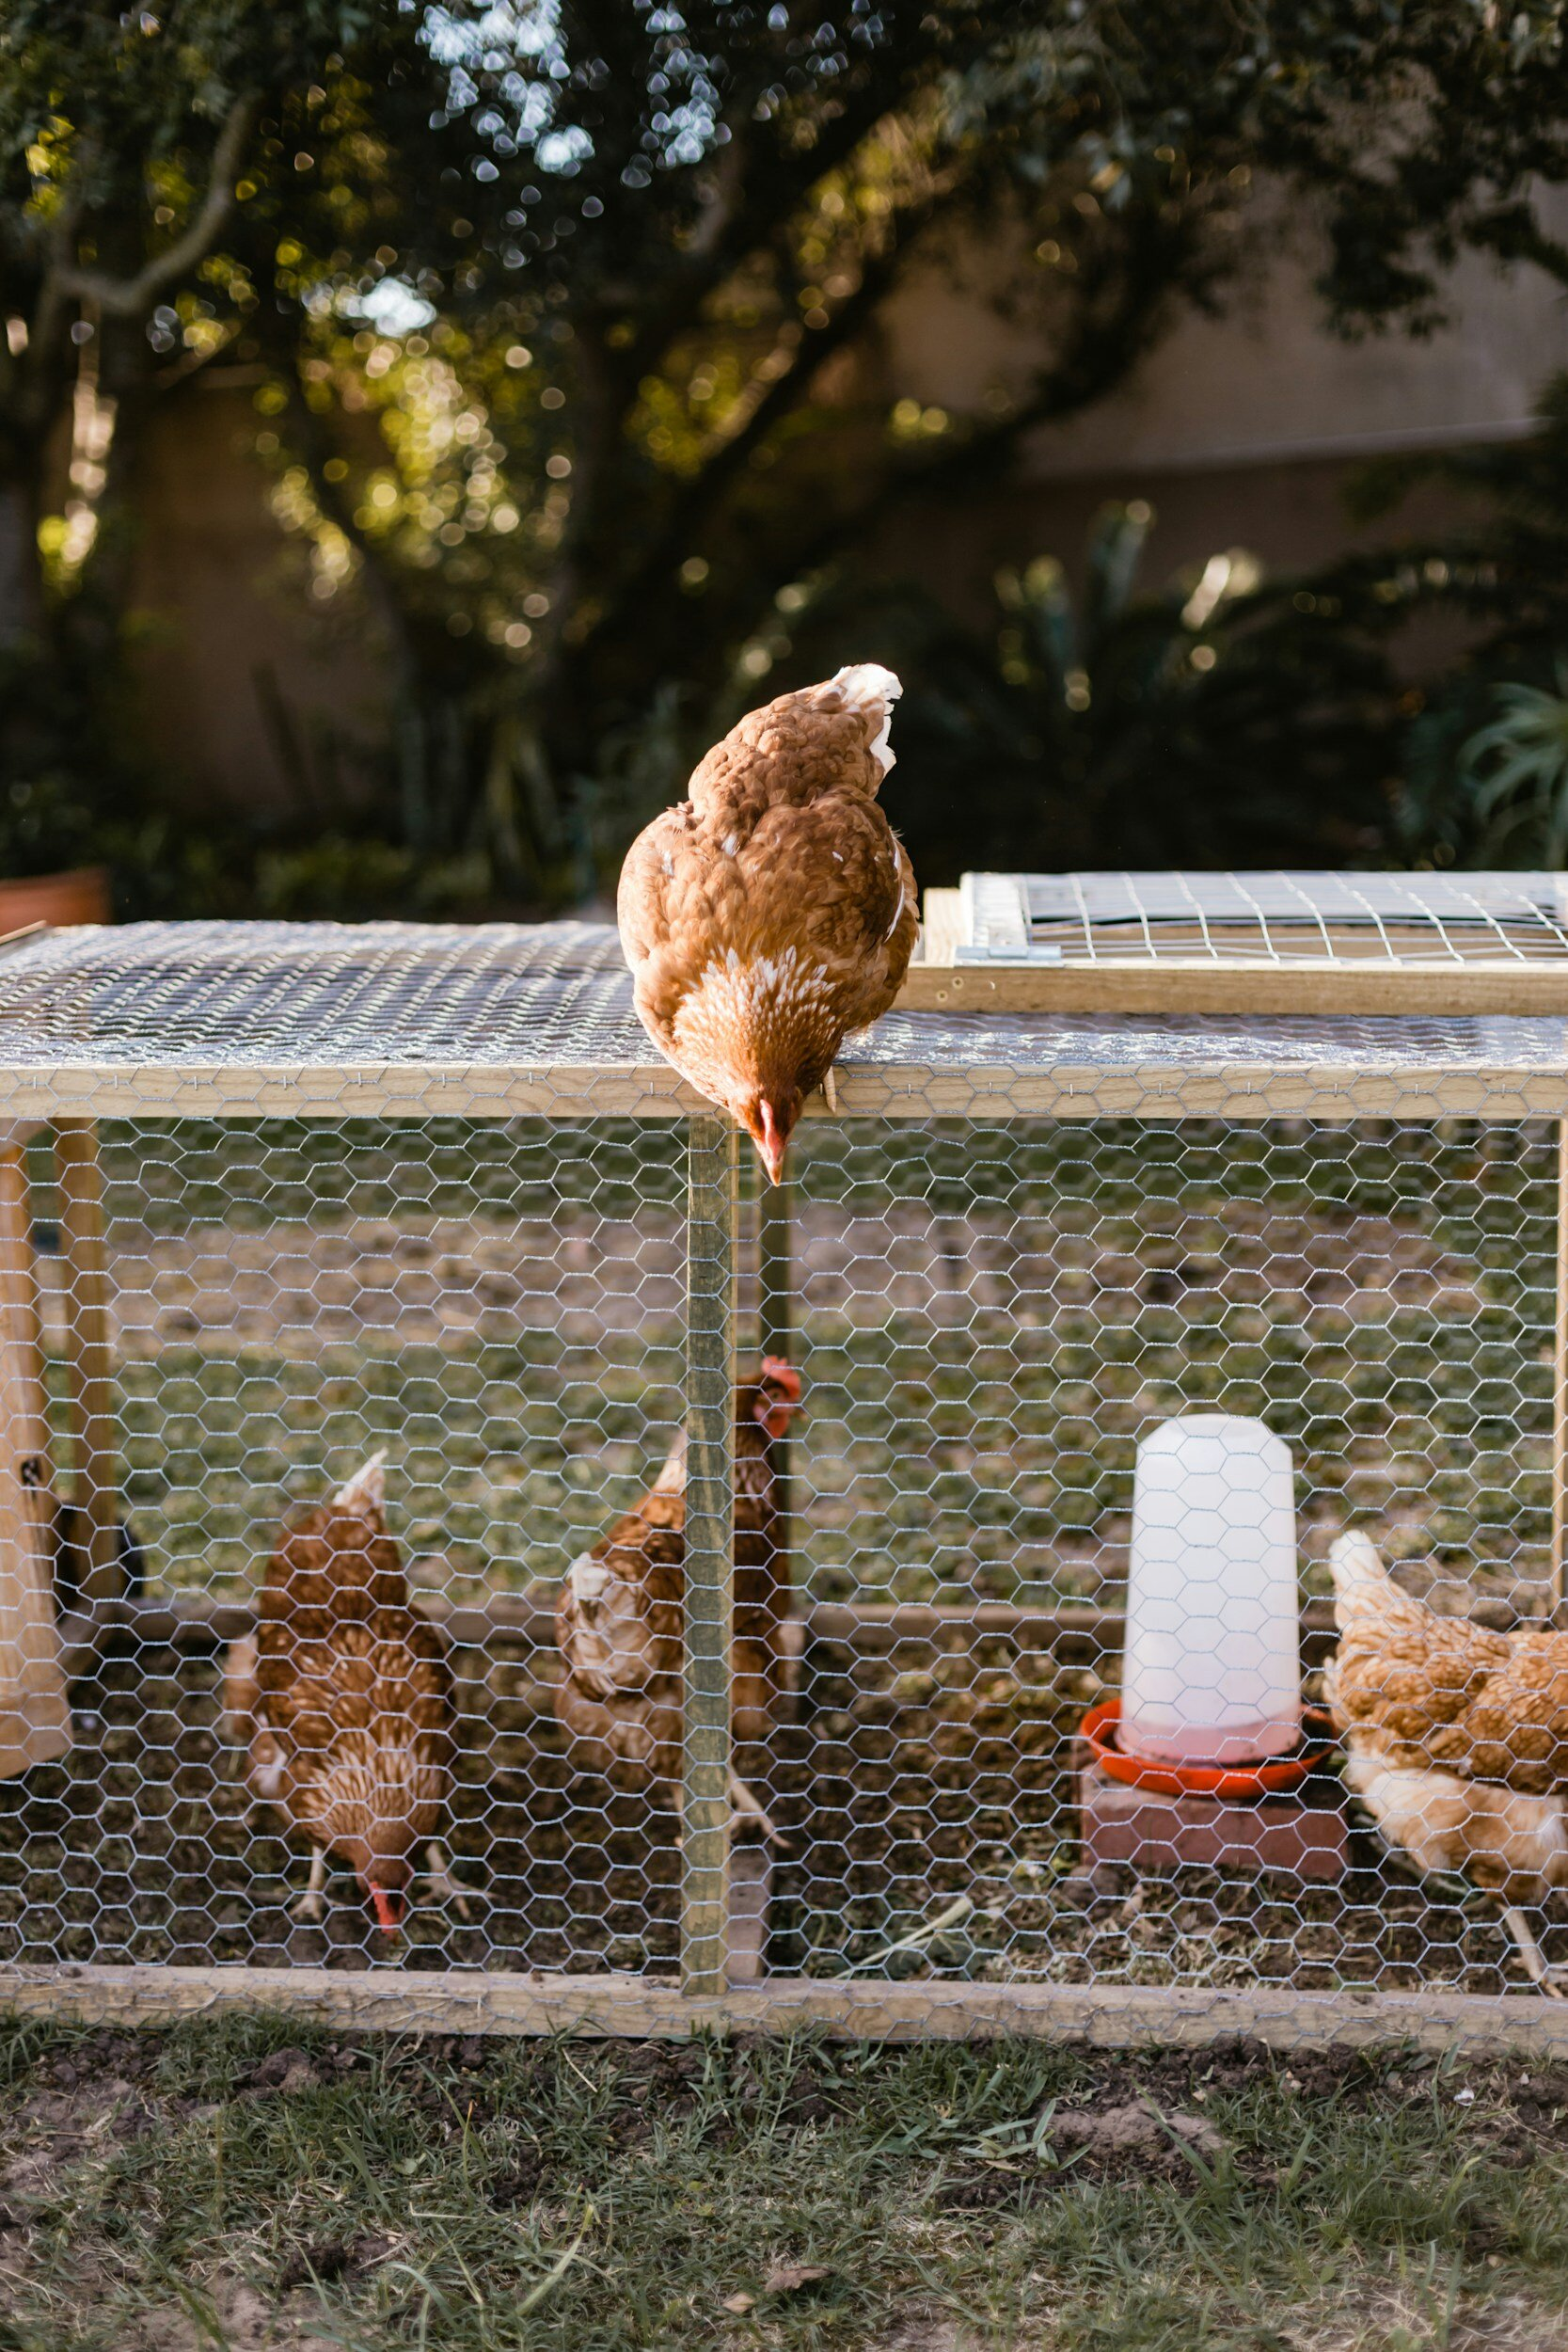
\includegraphics[width=0.85\textwidth]{./fig/image-asset.jpeg}
        \end{column}
    \end{columns}
\end{frame}

\begin{frame}
    \frametitle{Model Problem: Baking}
    \begin{itemize}
        \item Unknown underlying function $F$ %off top of head
            \pause
        \item Evaluating $F$ is expensive.
            \pause
        \item $F$ is smooth
            \pause
    \end{itemize}
    Solution: Iteratively evaluate $F$.
\end{frame}

\begin{frame}
    \frametitle{Algorithm: Overview}
    Given unknown function $F: \mathcal{X} \subseteq \mathbb{R}^{N} \to \mathbb{R}$, do the following loop
    \begin{enumerate}
        \item Given our beliefs about $F$, pick $\mathbf{x} \in \mathcal{X}$ with the most ``utility''.
            \pause
        \item Evaluate $F(\mathbf{x})$
            \pause
        \item Update our beliefs about $F$
            \pause
        \item Repeat
            \pause
    \end{enumerate}

    Our Bayesian optimization parameters are
    \pause
    \begin{itemize}
        \item Regression model to represent belief of $F$ given noisy observations $F(\mathbf{x}_1) \approx y_1, \dots, F(\mathbf{x}_N) \approx y_N$.
            \pause
        \item Measure of utility
    \end{itemize}
\end{frame}
\begin{frame}
    \frametitle{Parametric Regression}
    \begin{columns}
        \begin{column}{0.5\textwidth}
            \begin{center}
                Linear Regression
                \begin{equation*}
                    F(x) = \beta_1 x + \beta_0
                \end{equation*}

                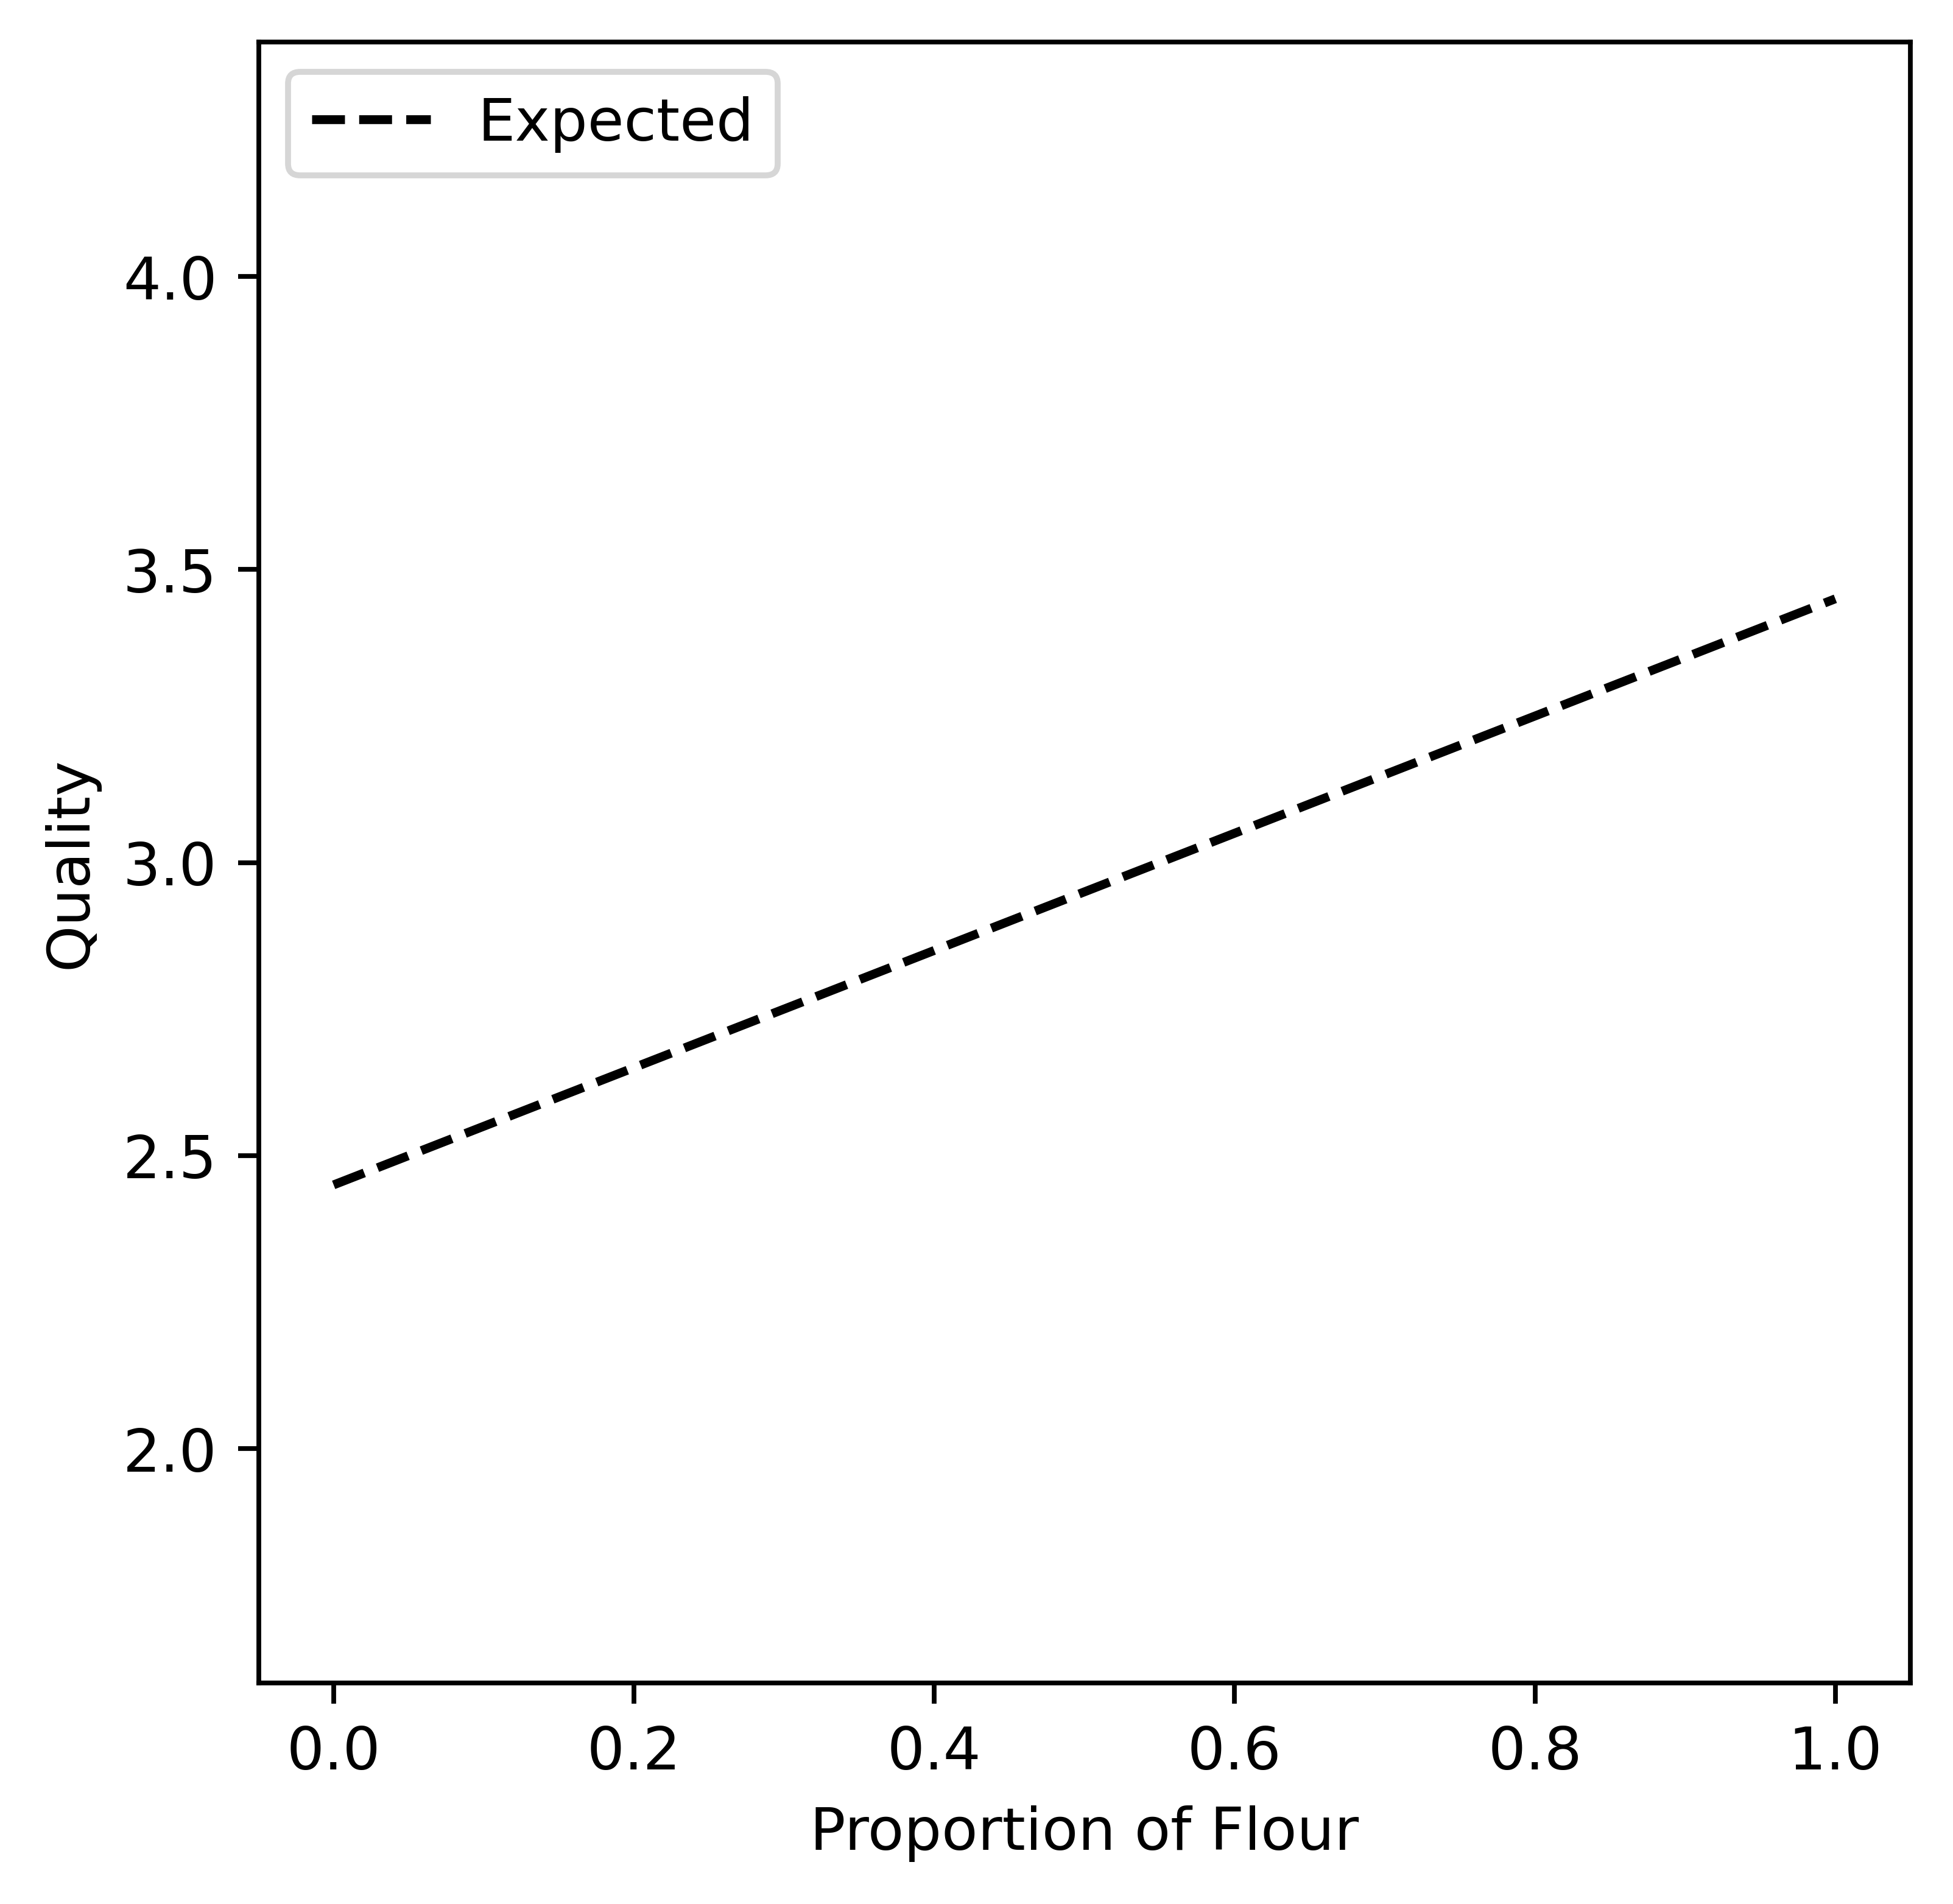
\includegraphics[width=\textwidth]{fig/linear.png}
            \end{center}
        \end{column}
        \pause
        \begin{column}{0.5\textwidth}
            \begin{center}
                Quadratic Regression
                \begin{equation*}
                    F(x) = \beta_2 x^2 + \beta_1 x + \beta_0
                \end{equation*}
                \includegraphics[width=\textwidth]{fig/quadratic.png}
            \end{center}
        \end{column}
    \end{columns}
\end{frame}
\begin{frame}
    \frametitle{Parametric Regression Doesn't Work}
    \begin{columns}
        \begin{column}{0.5\textwidth}
            \begin{center}
                Linear Regression
                \begin{equation*}
                    F(x) \neq  \beta_1 x + \beta_0
                \end{equation*}
                \includegraphics[width=\textwidth]{fig/linear-over.png}
            \end{center}
        \end{column}
        \begin{column}{0.5\textwidth}
            \begin{center}
                Quadratic Regression
                \begin{equation*}
                    F(x) \neq \beta_2 x^2 + \beta_1 x + \beta_0
                \end{equation*}
                \includegraphics[width=\textwidth]{fig/quadratic-over.png}
            \end{center}
        \end{column}
    \end{columns}
\end{frame}

\begin{frame}
    \frametitle{Nonparametric Regression}
    \begin{enumerate}
        \item Small changes in $\mathbf{x}$ probably cause small changes in $F(\mathbf{x})$.
            \pause
        \item The more we evaluate $F$ ``near'' $\mathbf{x}$, the more confident we are about $F(\mathbf{x})$.
    \end{enumerate}
\end{frame}

\begin{frame}
    \frametitle{Gaussian Processes}

    Uncountably infinite collection of r.v.
    $\{ F(\mathbf{x}) : \mathbf{x} \in \mathcal{X} \}$.

    \pause
    \begin{definition}[Gaussian Process]
        $F \sim \mathcal{GP}_{ \mathcal{X}}(m, \kappa)$ where
        \begin{align*}
            \mathbb{E}[F(\mathbf{x})] & = m(\mathbf{x}) \\
            \Cov[F(\mathbf{x}), F(\mathbf{x}')] & = \kappa(\mathbf{x}, \mathbf{x}')
        \end{align*}
        with
        \pause
        \begin{equation*}
            \begin{bmatrix}
                F(\mathbf{x}_1) \\
                \vdots \\
                F(\mathbf{x}_N) \\
            \end{bmatrix}
            \sim
            \mathcal{N}_{N}
            \left(
            \begin{bmatrix}
                    m(\mathbf{x}_1) \\
                    \vdots \\
                    m(\mathbf{x}_N) \\
                \end{bmatrix}
            ,
            \begin{bmatrix}
                    \kappa(\mathbf{x}_1, \mathbf{x}_1) & \dots & \kappa(\mathbf{x}_1, \mathbf{x}_N) \\
                    \vdots & \ddots & \vdots \\
                    \kappa(\mathbf{x}_N, \mathbf{x}_1) & \dots & \kappa(\mathbf{x}_N, \mathbf{x}_N) \\
                \end{bmatrix}
            \right).
        \end{equation*}
    \end{definition}
\end{frame}

\begin{frame}
    \frametitle{Radial Basis Function}
    \begin{center}
        \includegraphics[width=0.7\textwidth]{./fig/rbf}
    \end{center}
    \begin{equation*}
        \kappa_{\rbf}(\mathbf{x}, \mathbf{x}'; \sigma^2_f, \ell^2)
        = 
        \sigma^2_f \exp \left\{ - \frac{\lVert \mathbf{x} - \mathbf{x}' \rVert^2 }{ 2 \ell^2 } \right\}
    \end{equation*}
\end{frame}

\begin{frame}
    %interpret axis univariate GP y on (e.g. only ary amount of flour).
    % at this point, these are our belief.
    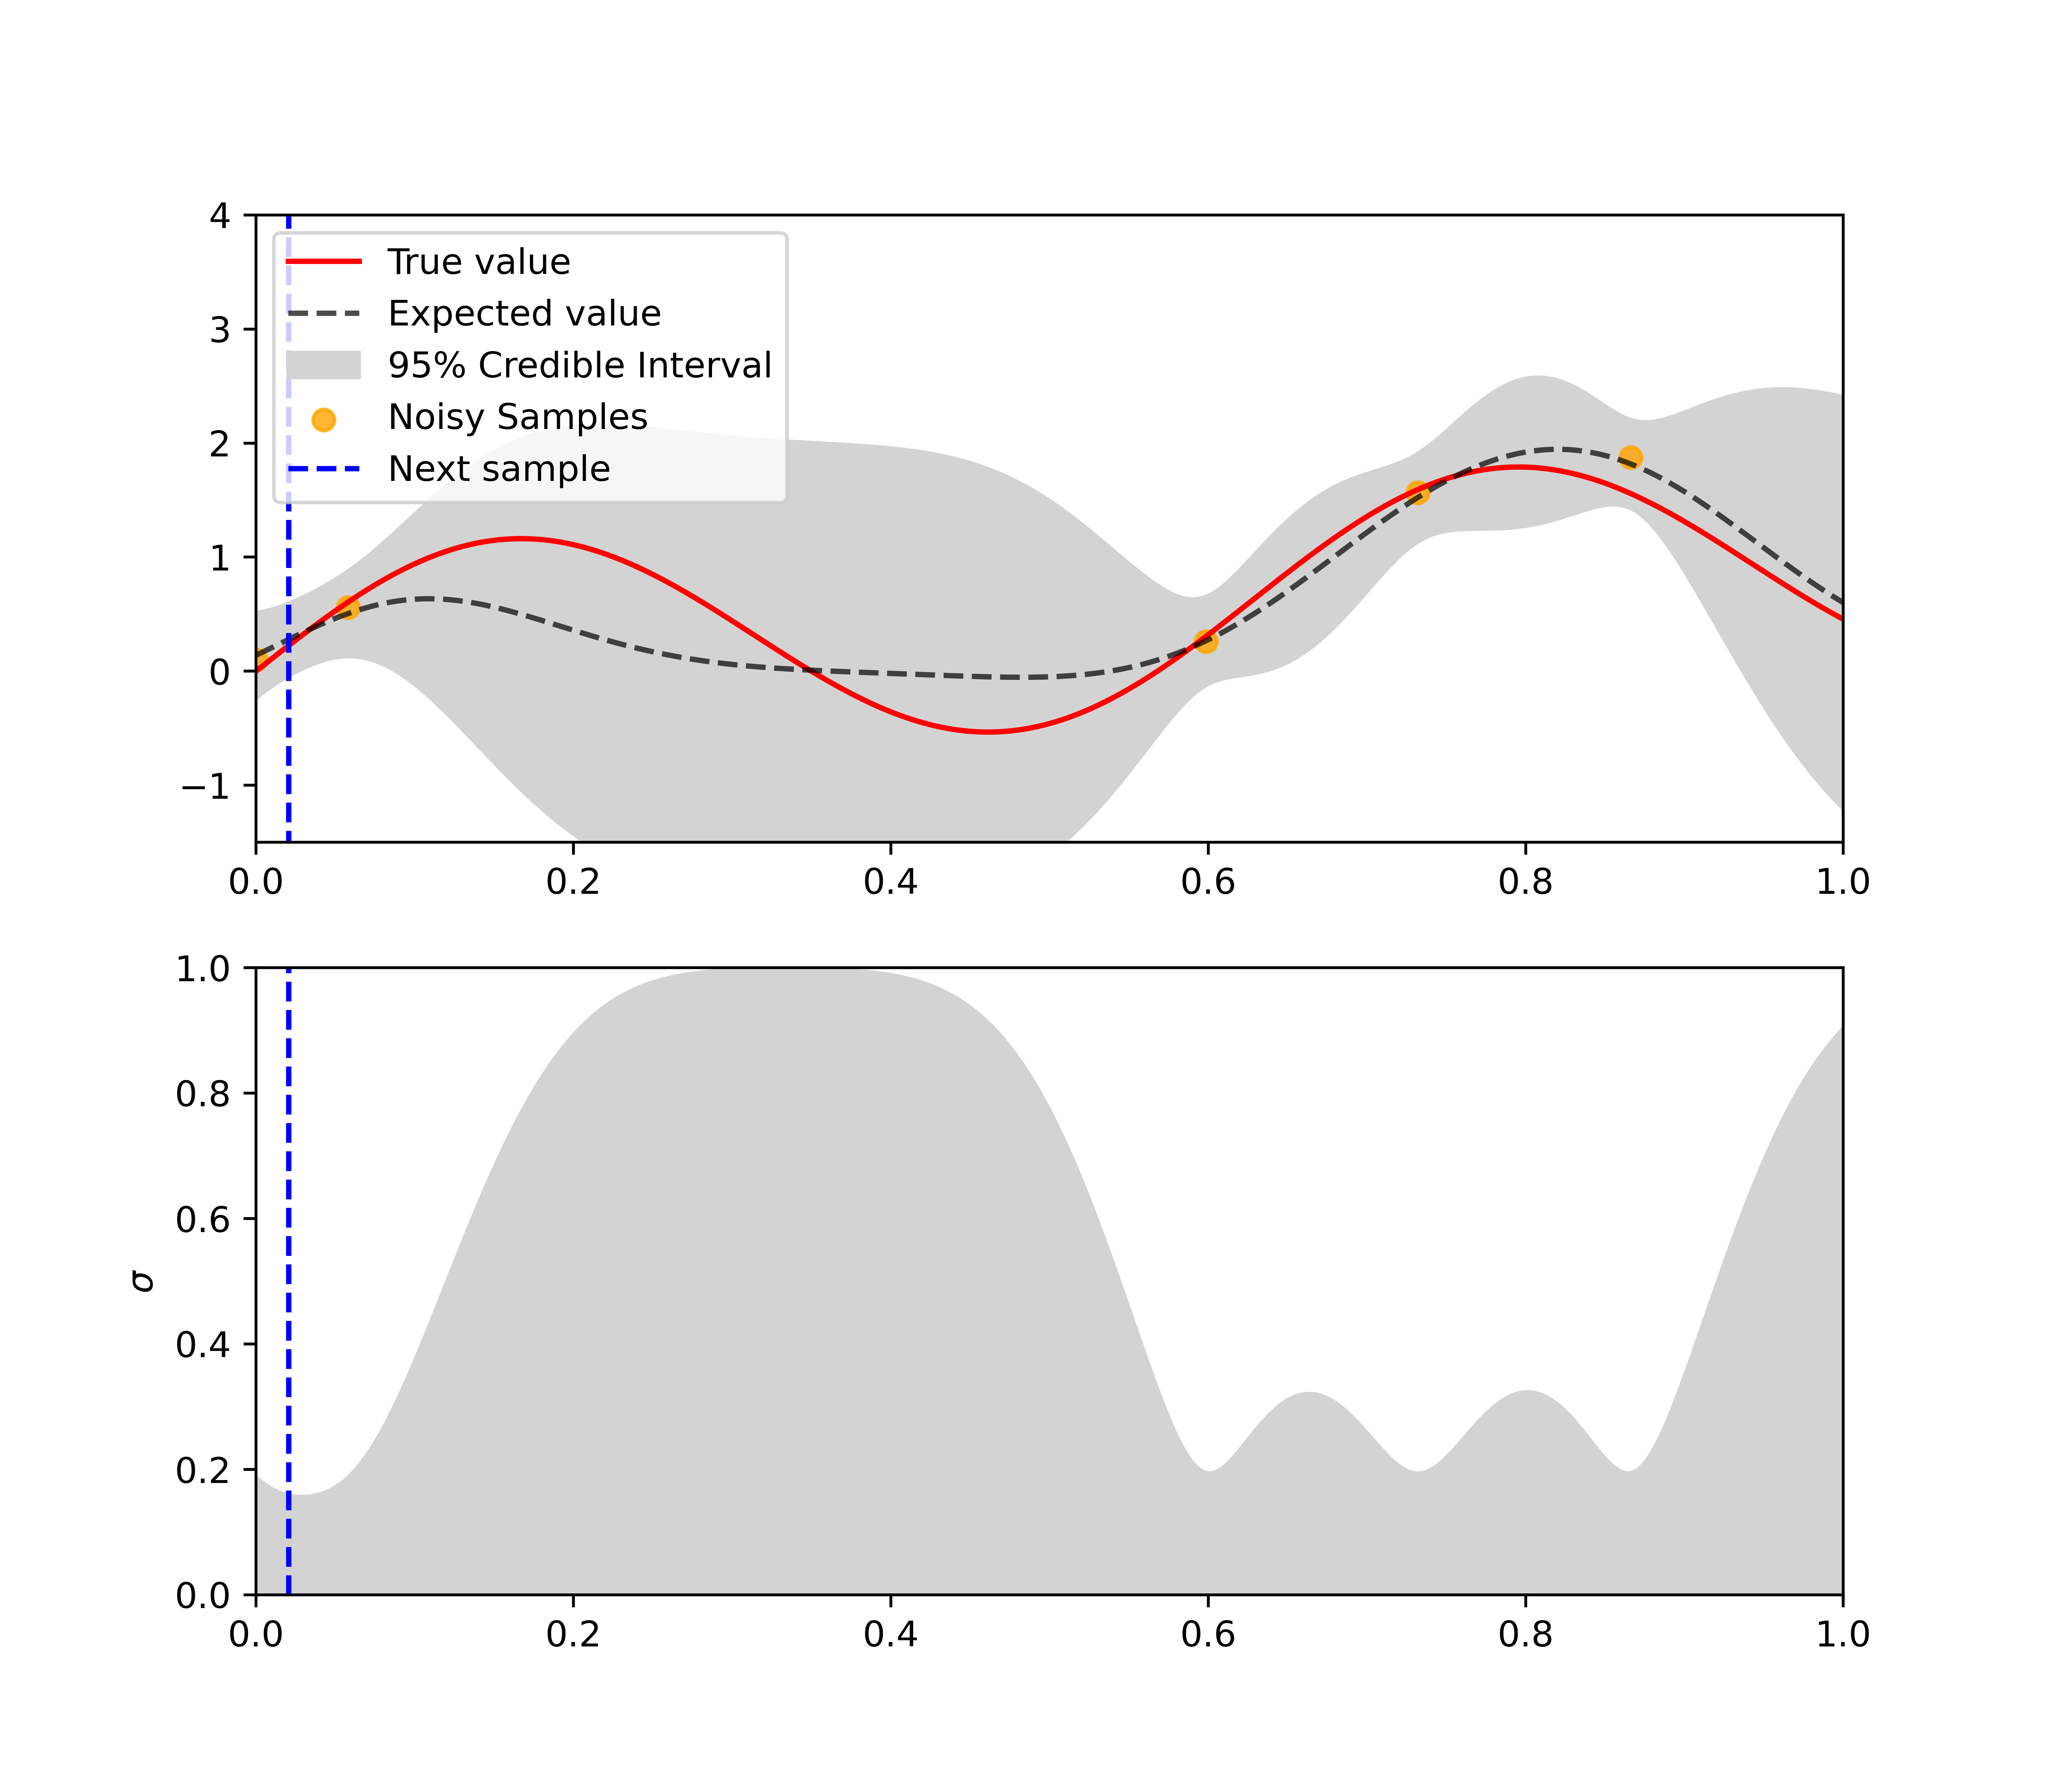
\includegraphics[width=\textwidth]{fig/sample_4.png}
\end{frame}

\begin{frame}
    \frametitle{Acquisition Functions}
    Given $\mathbf{x}$, how much ``utility'' do we get from evaluate $F(\mathbf{x})$?
    % reminder of what the goal is
    \begin{itemize}
        \item \textbf{Exploration}: want to know where the peaks are.
        \item \textbf{Exploitation}: want to understand how known peaks behave.
    \end{itemize}
\end{frame}

\begin{frame}
    \begin{definition}[PI]
        For some large $t^{*} \in \mathbb{R}$,
        \begin{align*}
            a_{\ppi}(\mathbf{x} | \mathcal{D}_N) & =
            P(F(\mathbf{x}) > t^{*} | \mathcal{D}_N) \\
            & = \Phi\left( \frac{ \mathbb{E}[F(\mathbf{x}) | \mathcal{D}_N] - t^{*} }{ \sqrt{\Var[F(\mathbf{x}) | \mathcal{D}_N] }}\right)
        \end{align*}
        where $\Phi$ is Gaussian CDF and $\mathcal{D}_N$ are the first $N$ observations.
        % pick the one to maximize
    \end{definition}
    \pause
    Then,
    \begin{equation*}
        \mathbf{x}_{N + 1} = \argmax_{\mathbf{x} \in \mathcal{X}} a_{\ppi}(\mathbf{x} | \mathcal{D}_{N})
    \end{equation*}
\end{frame}
\begin{frame}
    % and teh next place where we evaluate F.
    \includegraphics[width=\textwidth]{fig/sample_ei.png}
\end{frame}

\begin{frame}
    \begin{center}
        \includegraphics[width=0.8\textwidth]{fig/cake.png}
    \end{center}
\end{frame}

\begin{frame}
    \frametitle{Results}

    \includegraphics[width=0.47\textwidth]{fig/ys.png}
    \includegraphics[width=0.48\textwidth]{fig/progression.png}
\end{frame}

\begin{frame}
    \frametitle{Conclusion}
    Bayesian Optimization can help us find ``the best,'' even when the function is unknown.
\end{frame}

\begin{frame}
    \frametitle{Acknowledgements}
    \begin{itemize}
        \item Professor Tang
        \item My suitemates Ran, Megan, and Alex.
    \end{itemize}
\end{frame}
\end{document}
